In order to test the design outlined in Section~\ref{sec:rebuilding:design}, a software tool was produced.  The role of this tool is to:

\begin{enumerate}
    \item `Read' a seed corpus to construct a description of its metadata;
    \item Store this metadata as a description that is transferrable and portable;
    \item Replicate the input distribution of metadata by sampling from the web.
\end{enumerate}

This forms the basis of the `replication', `rescaling' and `distribution' scenarios specified in Section~\ref{sec:rebuilding:rationale:usecases}, as well as covering a superset of the features required for some simpler workflows (such as `repair').  This section details the design and architecture of the solution produced.


\subsection{Architecture}
The tool, named `ImputeCaT', is a small collection of command-line tools written using the Ruby programming language\footnote{\url{https://www.ruby-lang.org/en/}}. It is structured around two main executables: the former of these is called the Corpus ProfileR (hereafter `cpr'), and is responsible for reading a corpus, extracting its metadata, and serialising the resultant distribution to disk.  The latter reads, resamples, and attempts to retrieve documents matching an existing corpus profile---as it is seeking a gold standard, it is named the Golden Retriever (or simply `gr').

The separation of the tools at that stage offers many advantages: firstly the serialised corpus distribution acts as a file format, allowing a corpus to be passed between users, and secondly it offers a `DMZ' approach to information security: there is no mechanism for any (potentially sensitive or confidential) information from the original corpus to be used by the retrieval tool, except that which has been explicitly extracted.  Finally, this approach permits easy parallel execution of tools using a corpus description for read-only tasks.


Currently, both tools read descriptions of metadata type (and other resources) from a `profile' file.  This provides corpus-design-specific configuration data that would otherwise be impractical to enter through the command-line (for example, mappings from field names to metadata types).




\subsubsection{Document Description}
Documents are the sampling unit of ImputeCaT, and are used as atoms in sampling algorithms.  Each document is represented as a key-value store of metadata `names' (assigned using the profile description) and their respective values, along with the content that is being represented in the form of a plain text string.

This structure is used even where a document lacks text: building a corpus description from metadata will create a corpus with many documents, yet these will be populated solely by metadata fields and will have empty content elements.  Documents are mutable, and as they pass through the system they are liable to be edited in order to refine and change their contents according to a number of processes.




\subsubsection{Corpus Description}


\begin{figure}[h]
    \centering
    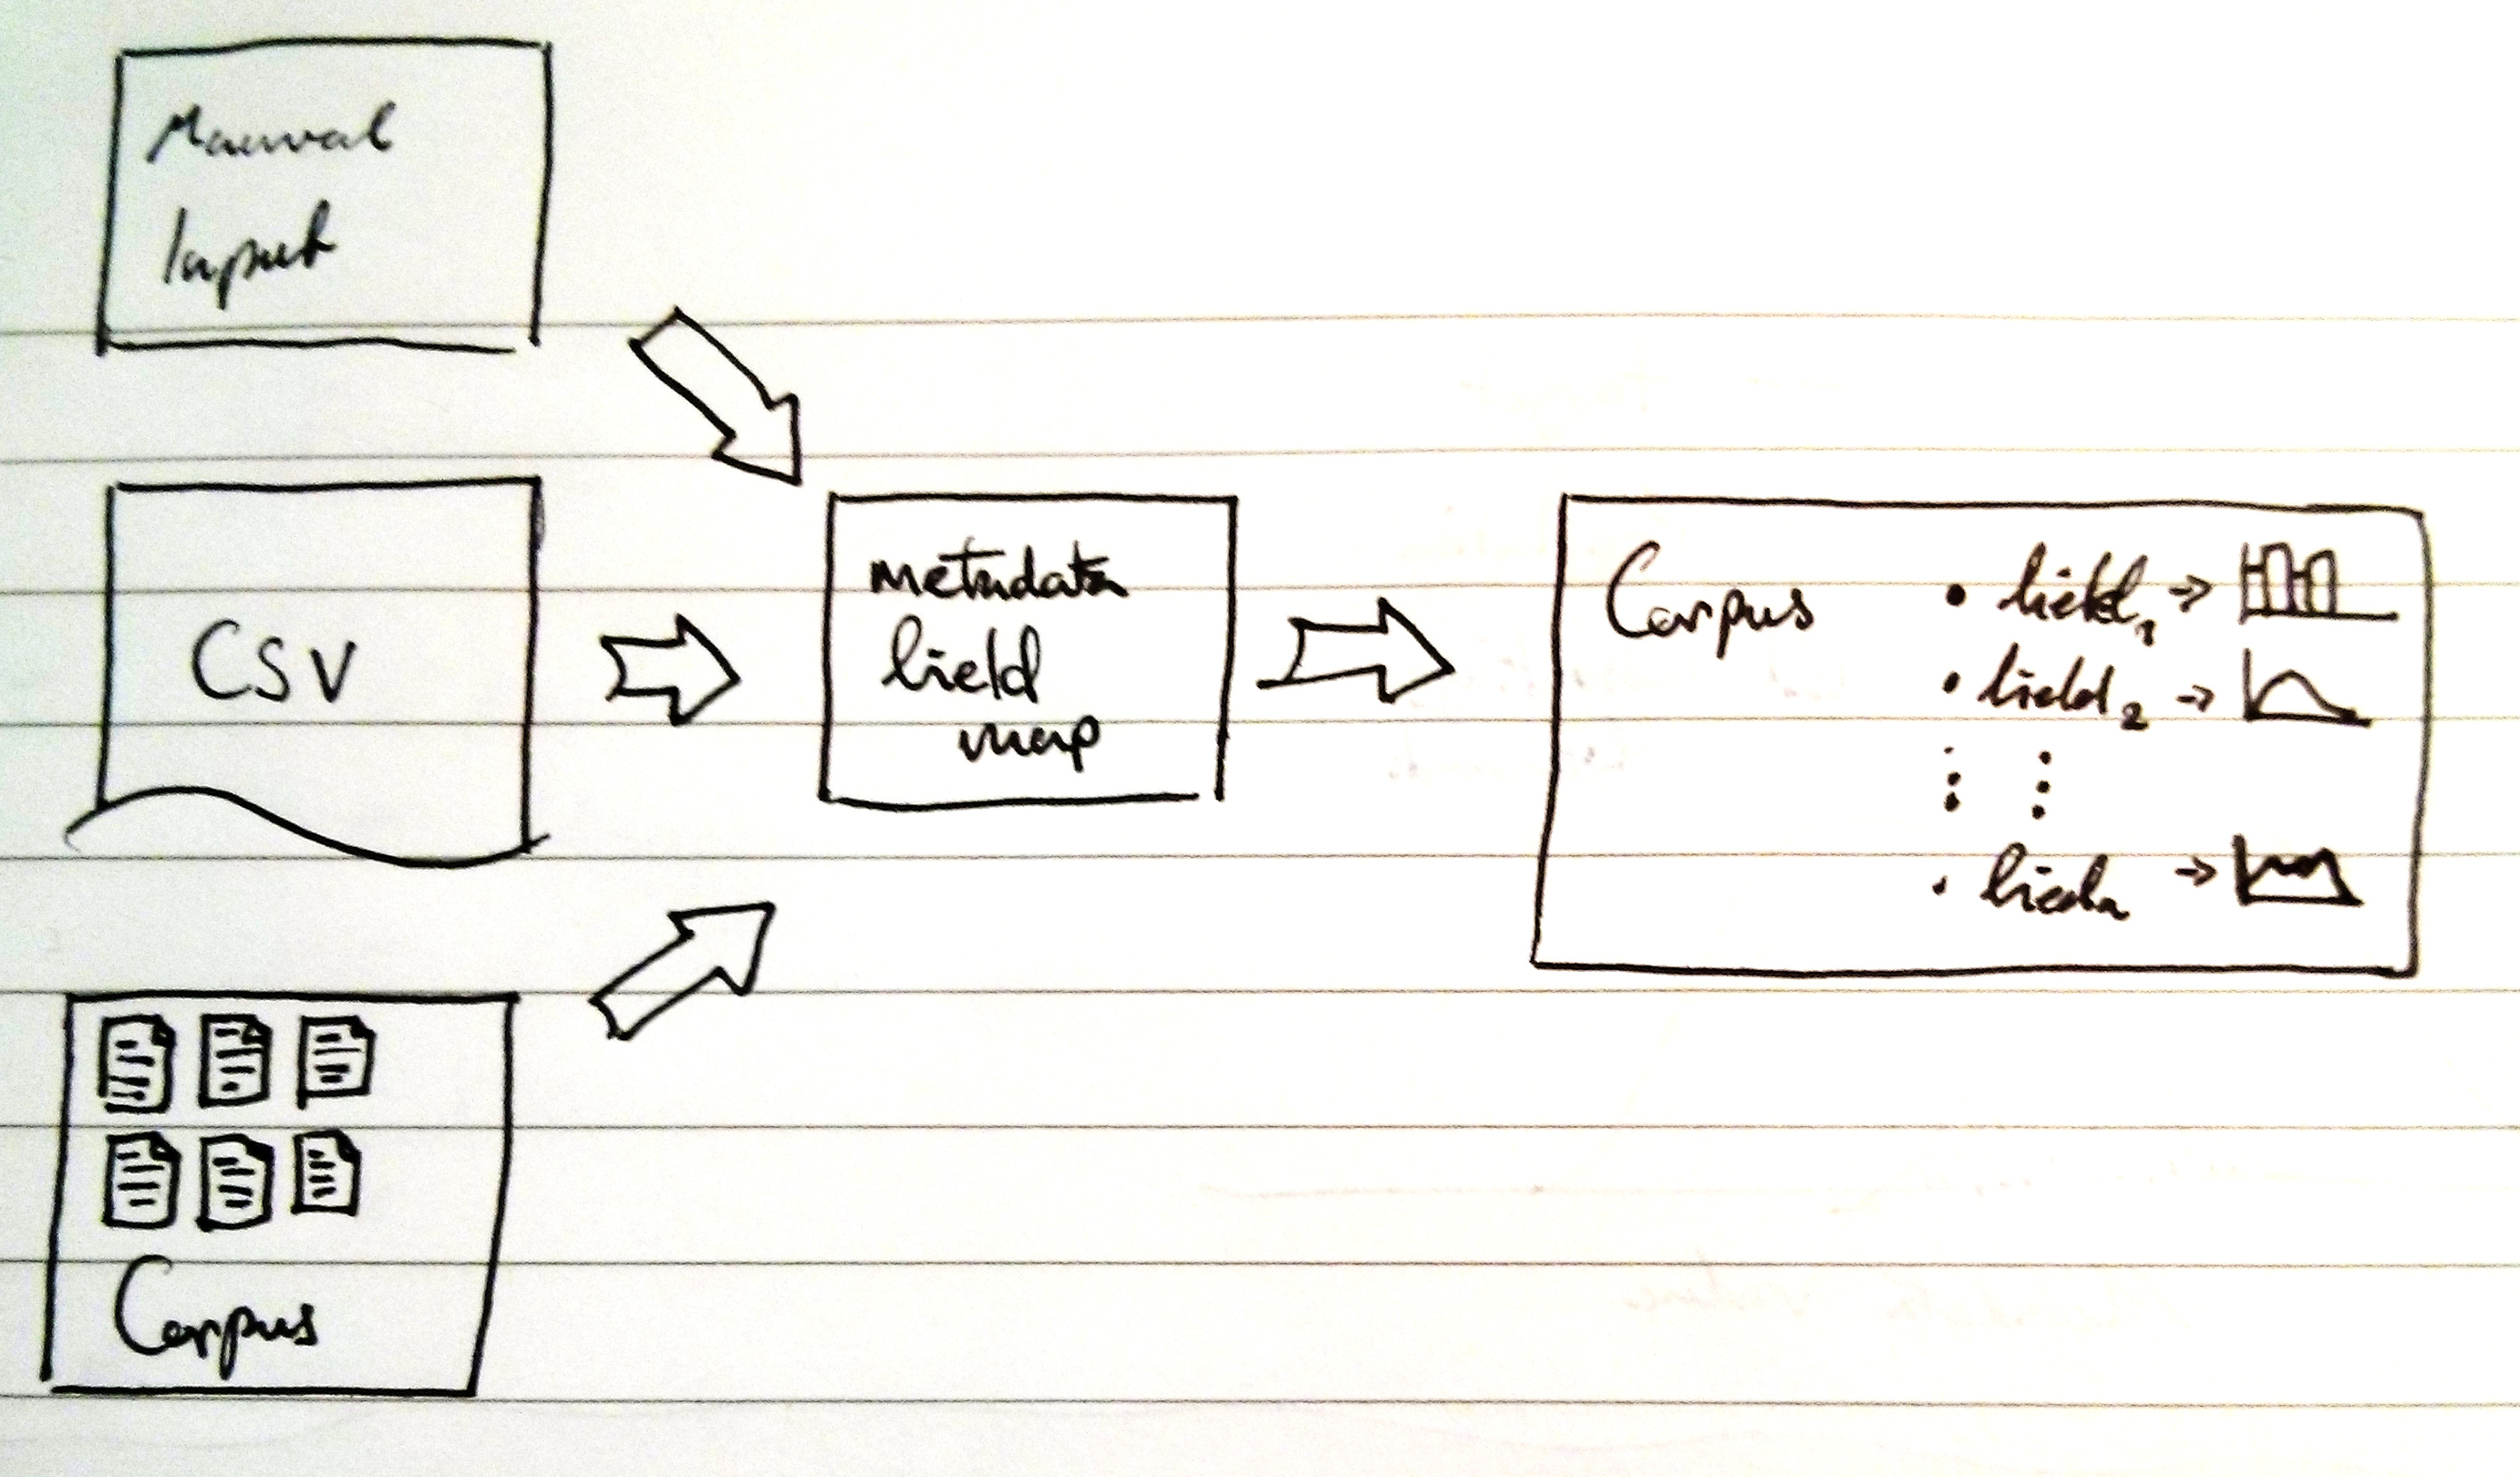
\includegraphics[width=0.8\textwidth]{rebuilding/loading-block}
    \caption{The objects involved in forming a corpus description}
    \label{fig:rebuilding:loading-block}
\end{figure}


The corpus description process is structured around gradually adding to a `corpus' object.  This object contains each document represented as a vector of metadata values, $d \in D; m \in d; m \in M$, along with marginal distributions for each (which are stored for optimisation purposes).


The distributions used for each metadata type are arbitrary, and may be controlled in a similar manner to priors in Bayesian inference in order to relax or modify the results.  Currently two systems for estimating the empirical distribution of data exist: the simpler of these represents discrete data by simply storing frequencies for each value observed.  A continuous form of this represents  distribution as a sum of Gaussian kernels---this is designed to disperse the observations and provide a more meaningful overview of the input data.  These distributions are specified in the profile document provided to `cpr'.

Each distribution object supports sampling at a given value $x$, returning $P[x | \text{seed corpus data}]$, and a \texttt{random} function that returns a random number following the distribution in question.  The discrete distribution implementation uses roulette sampling to implement this, and the smoothed continuous distribution identifies at random one of the contributing Gaussian function then samples from it using the Box-Muller transform\cite{box1958}.

The process of reading a corpus to describe it is one of loading document metadata from files.  As illustrated in Figure~\ref{fig:rebuilding:loading-block}, the values of metadata may be loaded from a corpus in CSV format, or from a manual description of the metadata required.  In addition to the metadata field values for each document, a mapping from CSV field names to metadata distributions is required, in order to define how each item of data is to be stored and manipulated.

It is possible at this stage to select distributions that artificially manipulate the metadata of a corpus, allowing users to `filter' or skew an existing corpus without manually editing each file prior to insertion.  This could be used to produce stochastic subcorpora, where the probability of undesirable documents is not eliminated but merely reduced, in effect rebalancing the corpus on-the-fly.  This is akin to two-phase stratified sampling, yet offers possibilities beyond simple weighting of each input document.

The selection of distributions is performed using the profile file, in a human-readable format.  This section of the profile currently maps CSV field names to instances of the distribution objects in question, as shown in Listing~\ref{lst:rebuilding:profile-lst}.  The parameter passed to the SmoothedGaussianDistribution constructor defines the standard deviation of the Gaussian distributions used, causing slight variation in sampling around each point.

{\small{}
\begin{lstlisting}[language=Ruby,caption={Field mappings in the BNC corpus profile.},label=lst:rebuilding:profile-lst]
PROFILE = {

  # ...

  # CSV fields mapped to their distribution type
  fields: {
    'GENRE'         => Impute::DiscreteDistribution.new(),
    'Word Total'    => Impute::SmoothedGaussianDistribution.new(30),
    'Aud Level'     => Impute::DiscreteDistribution.new(),
    'Language'      => Impute::DiscreteDistribution.new(),
  },
}
\end{lstlisting}
}

This approach allows the application of weights and control over the resampling process in a manner that is explicit and more efficient than implementing a different sampling algorithm for each modification.

As features are extracted from the seed corpus, they are assembled into a single document object and stored in the corpus.  A corpus is, then, a set of documents with an accompanying set of distribution objects that describe the marginal distributions of each dimension of metadata.

It is possible to design a corpus that has no documents, and is simply a description of desired marginal distributions, however, this approach will limit the power of the rest of the system as it is unable to model any interactions between metadata types.  For certain selections of metadata types, this may not be a strong assumption, however, many of the metadata types that can be extracted from existing corpora are designed to be useful to human analysts and are thus non-orthogonal.

It is also possible to import a corpus from text only, by running classifiers and heuristics to extract important metadata during the import.  This method requires access to the full text of the input corpus, but has the effect of making any errors symmetric with those of the rejection sampling phase of the retrieval tool.


\subsubsection{Resampling}
\label{sec:rebuilding:method:retrieval:resampling}

\begin{lstlisting}[language=,caption={Output from the conditional resampler, run on the BNC corpus.},label=lst:rebuilding:condsampler]
Selecting random document from #<Corpus:4:9506908>...
 - dims: 4, docs: 4054
 - dims: 3, docs: 1652 (Aud Level == med)
 - dims: 2, docs: 51 (GENRE == W_newsp_brdsht_nat_arts)
 - dims: 1, docs: 1 (Word Total == 1335)
\end{lstlisting}

Resampling is the process of producing a document with metadata values that are in some way related to an existing corpus object's distribution of documents.

ImputeCaT implements three different resampling algorithms:

\begin{itemizeTitle}
    \item[Marginal] This sampler selects metadata values at random from each marginal distribution, without conditioning upon any values.  This will ignore interaction effects between metadata and thus cause overdispersion in the sampled documents, however, it is possible to run this method on a corpus with no documents.

    \item[Conditional] The full conditional sampler selects a metadata dimension at random, selects a value from its distribution, and then produces a sub-corpus conditioned on this value.  This process is repeated until no dimensions remain, at which point the metadata values used are returned (as shown in Listing~\ref{lst:rebuilding:condsampler}).  Since a sub-corpus must be constructed at each iteration (in order to rebuild the remaining variables' marginal distributions), this process is possible only on corpora with knowledge of individual documents.
    
    \item[Partial Conditional] This sampler follows the same basic `selection and conditioning' iteration as the full conditional sampler, yet stops after a set number of iterations.  It behaves in a manner similar to that of a blocked Gibbs sampler, producing documents that converge to a similar distribution to the input yet with greater dispersion.
\end{itemizeTitle}

Due to smoothing applied to continuous distributions in a corpus, it is possible to sample at random a value that will return no documents for the conditioning phase of either conditional resampling mechanism: the solution to this is to provide a window width to the method, in which all documents will be selected, effectively providing a reverse function for the smoothing method.  Since the standard deviation of each Gaussian kernel making up the smoothed distribution is known, the window size can be set in such a way to guarantee a given probability of selection, for example, a value of $1.645\sigma$ would result in a 95\% chance of selecting at least one document.  Such effects are more likely the more input distributions are artificially processed for editorial reasons.  Note that this method is a compromise to make sampling tractable: actual Gaussian kernels extend to $x \pm \infty$, meaning we would need to consider every point in the distribution.

The `gr' tool uses the full conditional sampler exclusively: this provides the most accurate documents under the assumption that the `seed' corpus is already fairly complete.



% ----------------------------------------------------------------------------------


\subsection{Document Search \& Retrieval}
After loading the corpus description and profile from disk, the process of iteratively retrieving documents begins.  There are a number of different approaches to this task (as detailed in Section~\ref{sec:rebuilding:design:searching}): `gr' uses one that is designed to minimise interactivity during execution, in order to permit construction of arbitrarily large corpora with little effort.

The process of rebuilding a corpus is one of iterating the algorithm below until the size requirements are met:

\begin{enumerate}
    \item Sample a document from the seed corpus, known as the `prototype';
    \item Using a set of pre-defined search methods, select a set of candidate documents that is a superset of the prototype;
    \item Impute missing metadata values using context from the search system and document contents using a series of feature extractors;
    \item Identify and select the best candidate document by minimising distance in vector space (rejection sampling).
\end{enumerate}

The approach of scoring each candidate document after retrieval is arguably unnecessary if other retrieval methods are used: for example, manually selecting documents could prove so accurate for some metadata types that it need not be verified automatically (though some annotator agreement measures may result in a similar process to the above).

This rejection sampling method was selected in order to relax the precision requirements for each of the search methods.  In practice, each search method is likely to oversample somewhat from a population distribution which is unlikely to fit the seed corpus---the number of candidate documents selected ought to be proportional to the difference between the seed distribution and the population one.

Output is in the form of plaintext, along with stand-off documentation providing details of the metadata for each document.  Part of this metadata contains the prototype's details, in order to compute fit offline.



\subsubsection{Search Methods}
Methods used for searching are implemented as pluggable objects that accept a document to search for (and the names of any metadata field types they respect) and follow some procedure for retrieving candidate documents.

Search methods need not retrieve documents by searching for all metadata fields (though ideal, this is essentially not possible online), however, they should maximise variation in dimensions which they do not deliberately target in order to increase the coverage over the search space.  Use of multiple overlapping search strategies in construction of each candidate set ensures that each dimension of metadata is given an equal chance of being selected correctly.

It is desirable that these search methods cover as much of the possible search space as possible, such that they do not apply the bias illustrated in Figure~\ref{fig:rebuilding:population-bias}.  Nonetheless, selection of different search methods and heuristics will apply a set of assumptions that must ideally be aligned with the use of the resultant corpus: this is no different to any other corpus construction effort, except that this design explicitly enumerates and codifies this stage.  In the ideal case users will be able to select from a library of methods, each based upon empirically-validated theories---application of these would be able to adjust a corpus from one designer's set of assumptions to another, in order to ensure that it best fits a given use.

As documents are selected, their context must be passed on for use by heuristics and other processes.  This is accomplished via a special `meta' entry in the document object, which stores details such as HTTP headers and information on how to continue spidering from the document.  Some of the heuristics use these metadata for classification.

A web spidering system, Mechanize~\footnote{\url{http://wwwsearch.sourceforge.net/mechanize/}}, is available as a module for use with any retrieval methods.  Since it requires seed URLs, it does not constitute a retrieval method itself, however, it is the sole library used to retrieve and annotate web data, leaving behind a handle to the state of the spider in each document---using this it is possible to arbitrarily spider from any document that is currently in the system.  This behaviour is vital to retrieval of documents that are correct in only some dimensions, for example, from websites with the correct type and topic but lacking an appropriate word count.  Essentially, this mechanism allows other methods to exploit the clustered nature of the web to their advantage in seeking data.


\paragraph{i. Search}
Through the use of the Azure web services API~\footnote{\url{https://azure.microsoft.com/en-us/}} the Bing search engine can be used to retrieve URLs.  These may then be retrieved directly, or used as the starting point for a spider (see `Hybrid' below).

The Bing search engine allows for multiple search parameters, including language, selection by top level domain, and filtering using a number of heuristics to identify text types (for example, searching for the format of email headers).  These techniques allow for lookup of genres, though offer little control over some other features such as document length, which are typically of less interest to the average web user.  Nonetheless, for metadata which is searchable, the method of seeking a prototype offers a way to cut through the distortion applied by the search algorithms\footnote{Though this method is still subject to bias in their spidering algorithms.}.

The search mechanism in `gr' operates by detecting languages from metadata, searching the appropriate `market', and uses a series of pre-computed keyword lists to find matching genres.

Keywords for the system are passed as an argument in the corpus profile, and can thus be changed per-design to fit the classification used.  Both of the corpora used for testing in this thesis use Lee's BNC classification, for which log-likelihood-based keywords were computed.  Keywords are identified for use as search terms weighted by log likelihood values.


\paragraph{ii. Directory Search}
By using an existing web index, it is possible to map taxonomies directly to sets of links.  This has the distinct advantage of reliability and replicability, yet significantly reduces the potential pool of documents for selection.

The ability to use different indices (or search them) based upon another dimension of metadata makes this method suitable for use with very special-purpose corpora.  For example, one may search Project Gutenberg (a large repository of free ebooks) where the text type is `book', yet return to Bing search or DMOZ~\footnote{A.K.A. The open directory project, available at \url{http://www.dmoz.org/}} for less specialist documents.

Some of these resources may also fall offline, for example, a complete dump of Wikipedia and DMOZ are available and are used directly by ImputeCaT to find URLs.


\paragraph{iii. Hybrid}
The hybrid approach uses a search term or directory entry as a set of seed URLs from which to spider.

The most na\"ive implementation, implemented here, simply spiders a certain depth from each search URL\@.  It is also possible to select URLs to follow based on the prototype's values, either to seek a document directly or to maximise variation across non-controlled-for dimensions.

In his examination of different sources of URLs, Barbaresi identifies a lack of diversity in search engine results relative to sources such as DMOZ\cite{barbaresi2014finding}%
% p. 5
, whilst also noting that such directories underperform when applied to certain languages.  The prototype-seeking behaviour detailed here has the benefit of being able to switch between such approaches depending on language, maximising coverage for a given URL source.




\paragraph{iiv. Existing Fringe}
This mechanism simply searches the existing set of documents, left over from previous searches, for the closest match.  As all candidate documents are pre-ranked, this method requires no action.  It is equivalent to policies in genetic algorithm selection that retain portions of the population between generations.

Each relevant document in the fringe may also be used as the starting point for a spider, relying on the clustered nature of the web to maximise precision of retrieval.  


\subsubsection{Post-processing and Context}
After download, candidate documents must be converted to plaintext.  Processing modules are chainable, meaning that it is possible for each search method to construct a standard pipeline to normalise any contextual information and perform tasks such as boilerplate removal prior to document ranking and imputation using the heuristics.

\paragraph{i. Boilerplate Removal}
Boilerplate removal is performed by JusText\cite{pomikalek2013justext}.  Though currently this uses the bundled English stoplist, it would be possible to use the document context language attribute to automatically select a stoplist depending upon the input document.




\subsubsection{Heuristics}
Hailing from multiple sources, documents are unlikely to be annotated with sufficient metadata to permit comparison to the prototype.  It is thus often necessary to impute the values of metadata from what external variables are available (for example, meta-tags or HTTP headers) and the document content itself.

Unlike search strategies, heuristics need not consider the practical concerns of data sources, and are thus easier, simpler algorithms, often comprising simple classifiers or counts.  Nonetheless, error in these routines sums with other sources of dispersion: mechanisms for measuring the overall error of corpus documents (detailed below in Section~\ref{sec:rebuilding:method:errormeasure}) conflate these two sources.

Heuristics are also used to determine the `most similar' document to the prototype: each heuristic object harbours two methods: one to impute the value of a metadata key based on the document contents, and one to measure distance from one value to another.  For many heuristics this is a simple normalised difference between two numbers.


\paragraph{i. Genre}
Genres are imputed through the use of a keyword-based classifier.  This is one of the more challenging dimensions to impute due to its complexity, the importance of accurate detection (and thus corpus replication), and the ambiguity of classifications in many genre taxonomies.

The representation of genre used within ImputeCaT was selected to align with human-usable taxonomies, and as such is largely aligned with the BNC index\cite{lee2001genres}.  Selecting this taxonomy burdens any execution of the tool with various assumptions about the data and the desired output that therefore align with Lee's genre distinctions (and any inadequacies thereof).  This is a perfect example of the value of explicitly selecting and stating one's design through the corpus profiling tool.


The genre heuristic in this implementation uses keyword data to classify texts based on their content.  This is a rudimentary but reliable approach that doesn't require any consistency in web data retrieved (but also thus ignores any useful meta-information therein).


Rather than simply assuming the taxonomy used elsewhere, it would be possible to represent genre arbitrarily, either as a set of entropy measures against certain features, or in a manner more fitting of the source data.  This approach is valuable where the source documents are less well defined, or where particular control is needed over the composition of a corpus (such as frequency profiles for certain words).

One particular use of this approach would be the modelling of under-resourced languages using bottom-up detection of features, as in Sharoff's 2007 study\cite{sharoff2007classifying}.  As with all such approaches, however, the reliance on automatic feature detection strips away a large portion of the utility of genre definitions, in that they are often less easily understood by humans.  


There is some argument for this approach, however, when compared to the often context-based labels applied to the BNC\@.  The classifier in ImputeCaT is tasked with accurate identification of classes that are not particularly easy to separate by linguistic features.  One possible reason for this is their tendency to conflate topic with form: \variable{W\_email} and \variable{W\_hansard} are largely stylistic differentiations compared to \variable{W\_religion} and \variable{W\_ac\_medicine}.  The resultant classifier, following a multinomial na\"ive Bayes approach\cite{mccallum1998comparison}, is described in more detail in Chapter~\ref{sec:evaluation}.


The difficulty with which genre is classified makes a case for careful selection of metadata, and illustrates a compromise: often, the most operationalisable and useful metadata selection will not be easily understood by computers, and yet more synthetic features extracted from texts are often difficult to seek in an online environment that is designed specifically for human use.


\paragraph{ii. Audience Level}

\begin{table}[h]
    \center
    \begin{tabular}{|c|c|c|}
        \hline 
        Flesch reability score & BNC Audience level & Standard Deviation \\
        \hline 
        63 & Low & 14.4\\
        55 & Med & 12.7 \\
        47 & High & 12.4\\
        82 & (unclassified, speech) & 20.6 \\
        \hline
    \end{tabular}
    \caption{Target Flesch reading ease scores and their equivalent BNC categorisation.}
    \label{tab:rebuilding:method:fscore}
\end{table}
%Readability ranks: 
% -  low: 664  items, mean = 62.95293871760397, sd = 14.424512199650604, var = 208.06655219786907
% -  med: 1651 items, mean = 55.44412267430666, sd = 12.76812426643693,  var = 163.02499728317557
% - high: 820  items, mean = 47.70965585209567, sd = 12.445956325065204, var = 154.90182884543054
% -  ---: 914  items, mean = 82.02288020623476, sd = 20.6424573733852,   var = 426.111046412025


Reading ease metrics are used to estimate the `Audience Level' classification provided by Lee.  This takes the form of the Flesch reading ease score\cite{flesch1948new}, quantised through selection of the nearest target value as in Table~\ref{tab:rebuilding:method:fscore}.

Distance is normalised on this score by dividing the distance between classifications by the maximum distance possible between all classifications.  The score is thus output in terms of distance between categories: comparison of any `low' score to any `high' one will be equal regardless of the degree to which the original value is low or high.

Note that this categorisation is a design choice on behalf of the corpus builder: it is also possible to code the reading ease measure as a continuous value, which would offer more nuanced measurement of similarity.


\paragraph{iii. Word Count}
Words are counted by simply splitting the plaintext string on whitespace, and counting the parts.

Whilst this imputation algorithm is trivial, normalising the distance metric is not: the normalised distance between words score is provided by artificially imposing an upper bound beyond which the distance is simply registered as $1$.




\subsubsection{Measurement of Error}
\label{sec:rebuilding:method:errormeasure}
Notably, by scoring each document according to its target, it is possible to measure overall error for each metadata property as the corpus is being built.  In a unidimensional context this greatly simplifies the process of minimising error (since it is possible to adjust the seed distribution to compensate for errors on-the-fly), however, such comparisons would be intractable when applied to the intricate conditional distributions found in real-world corpora.



As documents are selected, it is possible to compute their sampling error by taking the difference between metadata values relative to the prototype.  This difference will be in units defined per metadata type, following a distribution that, in the ideal case, is uniform.

The error surface is, in reality, as intricate as the original distribution of documents: there is no way to compute errors for all conditions within the corpus without simply comparing documents.  To operationalise measures of total distance, therefore, we may summarise the error in a number of ways: 
% \td{make a mathematical notation for this}:

\begin{itemizeTitle}

    \item[Mean Error] This is simply the mean of all errors for each metadata item, and provides a coarse-grained measurement of the overall bias for a given dimension.  This measure is analogous to measuring the area under the difference between marginal distributions of the input and output distributions for a given metadata dimension.

    \item[Mean Squared Error] A sum of the squares of differences between each document and its prototype, this provides a dispersion measure that does not include direction.  This measure is commonly used to assess the quality of sampling, however, may not adequately represent the difficulties of sampling data online.

    \item[Uniformality of Residuals] Correlation between prototype and document metadata values evidences the responsiveness of search methods, and is testable using Mann-Whitney's U.%  Alternatively, the error surface for each dimension may be tested for uniformality.\td{formalise}

\end{itemizeTitle}


% \til{These ought to be decided upon rel. Ch6's methods}

If weighting the candidate document selection function, greater mean standard error should be observed on those dimensions with lower weights.








